\documentclass[11pt,a4paper]{article}
\usepackage[T1]{fontenc}
\usepackage[utf8]{inputenc}
\usepackage[spanish,es-noshorthands]{babel}
\usepackage{amsmath,amssymb,bm}
\usepackage{graphicx}
\usepackage{booktabs}
\usepackage{hyperref}
\usepackage{siunitx}
\usepackage{geometry}
\geometry{margin=2.4cm}
\graphicspath{{../../results/tmm/}{../../figures/}}
\hypersetup{colorlinks=true,linkcolor=black,citecolor=blue,urlcolor=blue}

\title{Reimplementación computacional de plasmon-polaritones\\
en superredes fotónicas Fibonacci de metamaterial}
\author{Emanuel Orozco Gallego}
\date{31 de agosto de 2026}

\begin{document}
\maketitle

\begin{abstract}
Se presenta una reimplementación completa, reproducible y verificable del artículo
E.~Reyes-Gómez \textit{et al.}, Phys.\ Rev.\ B \textbf{81}, 153101 (2010).
El modelo se resuelve con el método de matriz de transferencia a incidencia oblicua,
sin FDTD ni elementos finitos. Se reconstruyen las secuencias de Fibonacci del paper
($F_0=F_1=1$), el Drude sin pérdidas y la relación $\cos(kL_m)=R_m$.
Las Figuras~1--5 del original se reproducen a partir de las ecuaciones publicadas.
El número de modos plasmon-polaritón coincide con $F_{m-2}$ en todos los casos
comprobados ($m=3,4,5,6$). La Figura~6 se calcula con parámetros inferidos porque
el caption original está incompleto: el eje vertical es frecuencia y cada región
rellena es una subbanda permitida frente a $\theta$, no una curva de $\Delta\nu$.
Se documentan las ambigüedades del paper, en particular la omisión de $\omega/c$ en $q$.
\end{abstract}

\tableofcontents
\newpage

\section{Introducción}

El artículo original estudia plasmon-polaritones magnéticos en una superred unidimensional
cuya celda elemental es una generación de Fibonacci $S_m$ de aire y metamaterial Drude.
El presente trabajo no es una paráfrasis de ese Brief Report: es una
\textit{reproducción científica computacional} que parte de las ecuaciones, implementa el
TMM, genera datos y figuras, y compara con el impreso.

Fuente primaria: el PDF de cuatro páginas. Donde el texto es incompleto se etiqueta
explícitamente la inferencia. La Ref.~\cite{Reyes2009EPL} (mismo grupo, citada como Ref.~16
del original) se usa solo para restaurar $q=(\omega/c)n_A\sin\theta$ y la convención
$e^{i(qx-\omega t)}$.

\section{Fundamentos físicos}

\subsection{Cristales fotónicos y gap $\langle n\rangle=0$}
En superredes que alternan índice positivo y negativo aparece un gap no Bragg asociado a
índice promedio nulo, esencialmente invariante de escala~\cite{Li2003,Bruno2008}.

\subsection{Metamateriales}
El medio B se describe como material de índice negativo en el intervalo en que
$\varepsilon_B<0$ y $\mu_B<0$, con respuestas tipo Drude~\cite{Veselago1968,Pendry1996,Pacheco2002}.

\subsection{Plasmon-polaritones}
A incidencia oblicua, el campo magnético TE tiene componente a lo largo de $z$ y acopla
con el plasmón magnético de volumen ($\mu_B=0$)~\cite{Reyes2009EPL}. A $\theta=0$ ese acoplamiento
desaparece.

\subsection{Superredes de Fibonacci}
La celda no es el dímero $AB$ sino $S_m$. La cuasiperiodicidad interna destruye la coherencia
espacial de largo alcance y fragmenta los modos en un espectro tipo Cantor~\cite{Kohmoto1983}.

\section{Modelo físico}

\subsection{Geometría}
Crecimiento a lo largo de $z$. Celda $S_m$ de bloques A (espesor $a$) y B (espesor $b$),
repetida periódicamente. En todas las figuras, $a=b=12\,\mathrm{mm}$.

\subsection{Secuencia de Fibonacci}
\begin{equation}
S_m=S_{m-1}S_{m-2},\qquad S_0=B,\quad S_1=A,
\end{equation}
con $F_0=F_1=1$ y $L_m=F_{m-1}a+F_{m-2}b$. Entonces $S_3=ABA$, $S_4=ABAAB$,
$N_B=F_{m-2}$.

\subsection{Materiales}
Aire: $\varepsilon_A=\mu_A=1$. Metamaterial (eq.~10 del original):
\begin{equation}
\varepsilon_B(\omega)=1-\frac{\omega_e^2}{\omega^2},\qquad
\mu_B(\omega)=1-\frac{\omega_m^2}{\omega^2}.
\end{equation}
Sin pérdidas. $\nu=\omega/2\pi$ es la magnitud graficada en GHz.
Figs.~1--2: $\omega_e/2\pi=\omega_m/2\pi=3\,\mathrm{GHz}$.
Figs.~3--5: $\omega_e/2\pi=3\,\mathrm{GHz}$, $\omega_m/2\pi=1\,\mathrm{GHz}$.

\section{Formulación electromagnética}

Para TE, $E$ es paralelo a las interfaces. La eq.~(1) del original es la Helmholtz
\begin{equation}
\frac{d}{dz}\Bigl[\frac{1}{\mu}\frac{dE}{dz}\Bigr]
=-\varepsilon\Bigl[\frac{\omega^2}{c^2}-\frac{q^2}{n^2}\Bigr]E,
\end{equation}
con $n=\sqrt{\mu}\sqrt{\varepsilon}$. El vector
$\Psi=(E,\,\mu^{-1}dE/dz)$ es continuo.
TM se obtiene sustituyendo $\mu\to\varepsilon$ en el factor de $R_2$.

El paper escribe $q=n_A\sin\theta$. Eso es adimensional, incompatible con $Q$.
Se implementa
\begin{equation}
q=\frac{\omega}{c}n_A\sin\theta,
\qquad
Q_{A,B}=\sqrt{\frac{\omega^2}{c^2}n_{A,B}^2-q^2}.
\end{equation}
$c=299\,792\,458\,\mathrm{m/s}$ (no especificado en el original).

\section{Método de matriz de transferencia}

La matriz de capa, reconstruida de $\Psi$ y validada contra las eqs.~(7)--(9), es
\begin{equation}
M=\begin{pmatrix}
\cos(Qd) & (\chi/Q)\sin(Qd)\\
-(Q/\chi)\sin(Qd) & \cos(Qd)
\end{pmatrix},
\end{equation}
con $\chi=\mu$ (TE) o $\chi=\varepsilon$ (TM) y $\det M=1$.
Si $S_m=X_1\cdots X_N$ de izquierda a derecha,
$T_m=M_N\cdots M_1=T_{m-2}T_{m-1}$.
La semitraza $R_m=\frac12\mathrm{Tr}(T_m)$ cumple
$R_m=2R_{m-1}R_{m-2}-R_{m-3}$~\cite{Kohmoto1983}.
Bandas: $\lvert R_m\rvert\le 1$; gaps: $\lvert R_m\rvert>1$.
En la primera zona, $kL_m/\pi=\arccos(R_m)/\pi\in[0,1]$.

\section{Implementación computacional}

Biblioteca \texttt{fibonacci\_tmm} en Python~3.14, NumPy, con parámetros en YAML.
Dos caminos independientes para $R_m$: producto de matrices y recurrencia; coinciden
dentro de $10^{-8}$ hasta $m=7$. Tests: 110 casos, 3 omitidos ($k>m$ en una identidad).
Tolerancia de banda: $\lvert R\rvert\le 1+10^{-12}$, documentada.

\section{Reproducción de resultados}

Todas las figuras de esta sección se generaron con
\texttt{python scripts/tmm/figure\_0N.py}, sin edición manual.

\subsection{Figura 1}
Parámetros: $\nu_e=\nu_m=3\,\mathrm{GHz}$, $S_3$ y $S_4$,
$\theta=0,\pi/12,\pi/6,\pi/3$.
A $\theta=0$, $\varepsilon_B(\omega)=\mu_B(\omega)$ implica adaptación de impedancia
con el aire: no hay gaps ($\lvert R\rvert\le 1$ en todo el barrido). El gap
$\langle n\rangle_m=0$ está cerrado en
$\nu=3\sqrt{F_{m-2}/F_m}\,\mathrm{GHz}$ ($1.732$ para $m=3$, $1.897$ para $m=4$).
A $\theta\neq 0$ se abren gaps no Bragg y polaritónicos.
Las curvas se cortan en los gaps ($|R_m|>1$) y en saltos de $k$ para no unir
ramas distintas con una recta horizontal, que era el artefacto que rellenaba
el panel a baja $\nu$. Concordancia: \textbf{buena}.

\begin{figure}[ht]
\centering
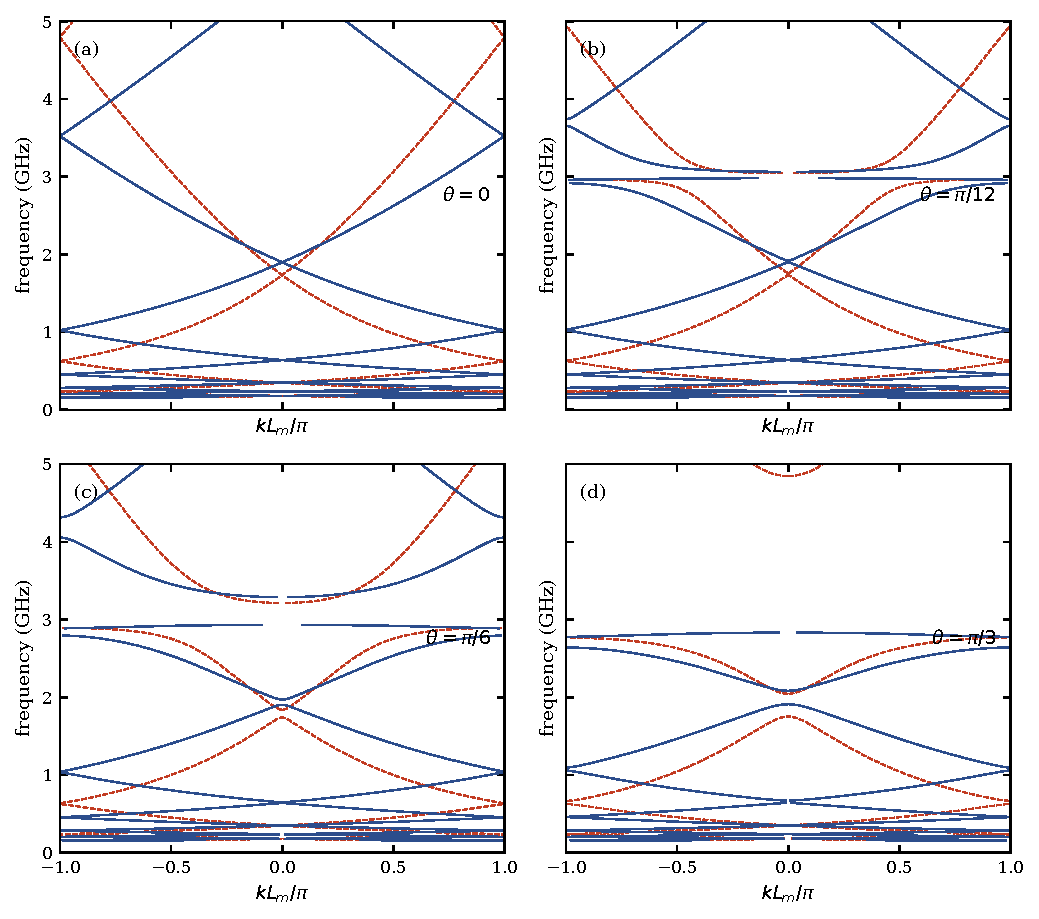
\includegraphics[width=0.95\linewidth]{figure_01/output/figure_01.pdf}
\caption{Reproducción de la Fig.~1. Dispersión TE para $S_3$ (discontinuo) y $S_4$ (continuo).
Script: \texttt{scripts/tmm/figure\_01.py}.}
\end{figure}

\subsection{Figura 2}
$\theta=\pi/3$, ventana $2$--$4\,\mathrm{GHz}$. Detección automática de subbandas:
$m=3,4,5,6$ $\to$ $1,2,3,5=F_{m-2}$ modos. Concordancia: \textbf{excelente}.

\begin{figure}[ht]
\centering
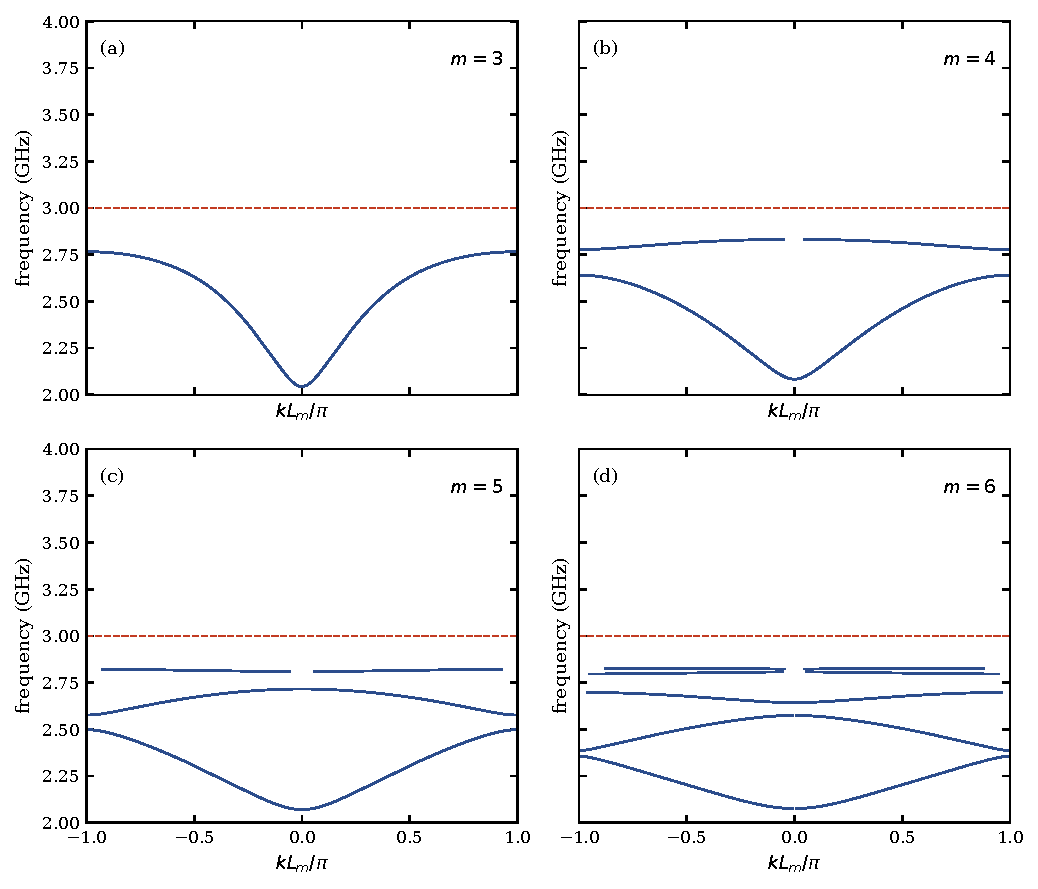
\includegraphics[width=0.95\linewidth]{figure_02/output/figure_02.pdf}
\caption{Reproducción de la Fig.~2. El número de ramas bajo $\nu_m=3\,\mathrm{GHz}$ es $F_{m-2}$.}
\end{figure}

\subsection{Figura 3}
$\nu_m=1\,\mathrm{GHz}$ cae en el gap $\langle n\rangle=0$. A $\theta=0$ no hay polaritón
plano en $1\,\mathrm{GHz}$; a $\theta\neq 0$ aparece una banda casi plana, como en el
original (el PRB no dibuja una línea de referencia en esta figura).
Concordancia: \textbf{buena}.

\begin{figure}[ht]
\centering
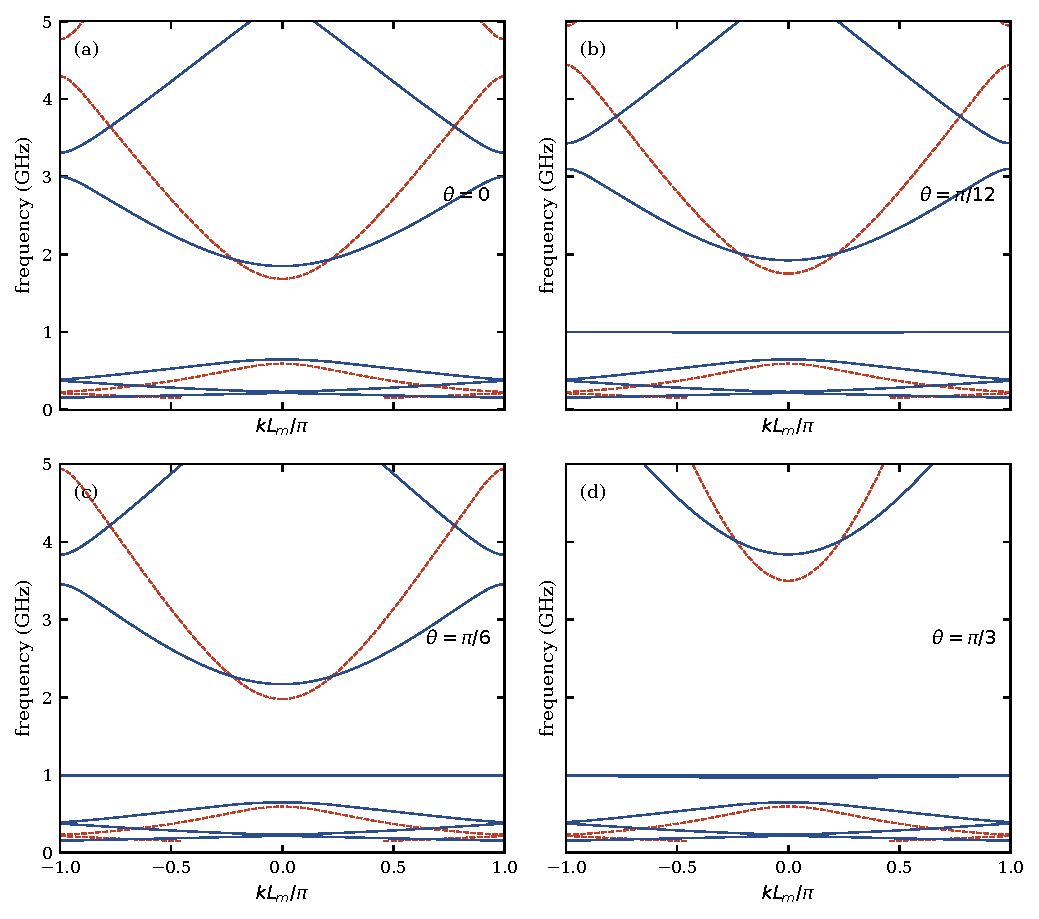
\includegraphics[width=0.95\linewidth]{figure_03/output/figure_03.pdf}
\caption{Reproducción de la Fig.~3. Como la Fig.~1, con $\omega_m/2\pi=1\,\mathrm{GHz}$.}
\end{figure}

\subsection{Figura 4}
Zoom. $m=3$: una subbanda. $m=4$: dos.
Anchos numéricos: $\theta=\pi/12$, $\Delta\nu\approx 4.51\,\mathrm{MHz}$ ($m=3$);
$\theta=\pi/3$, $\Delta\nu\approx 33.1\,\mathrm{MHz}$. El ancho crece con $\theta$,
como en el original ($\sim 5$ y $\sim 40\,\mathrm{MHz}$ leídos a ojo del impreso).
Concordancia: \textbf{excelente}.

\begin{figure}[ht]
\centering
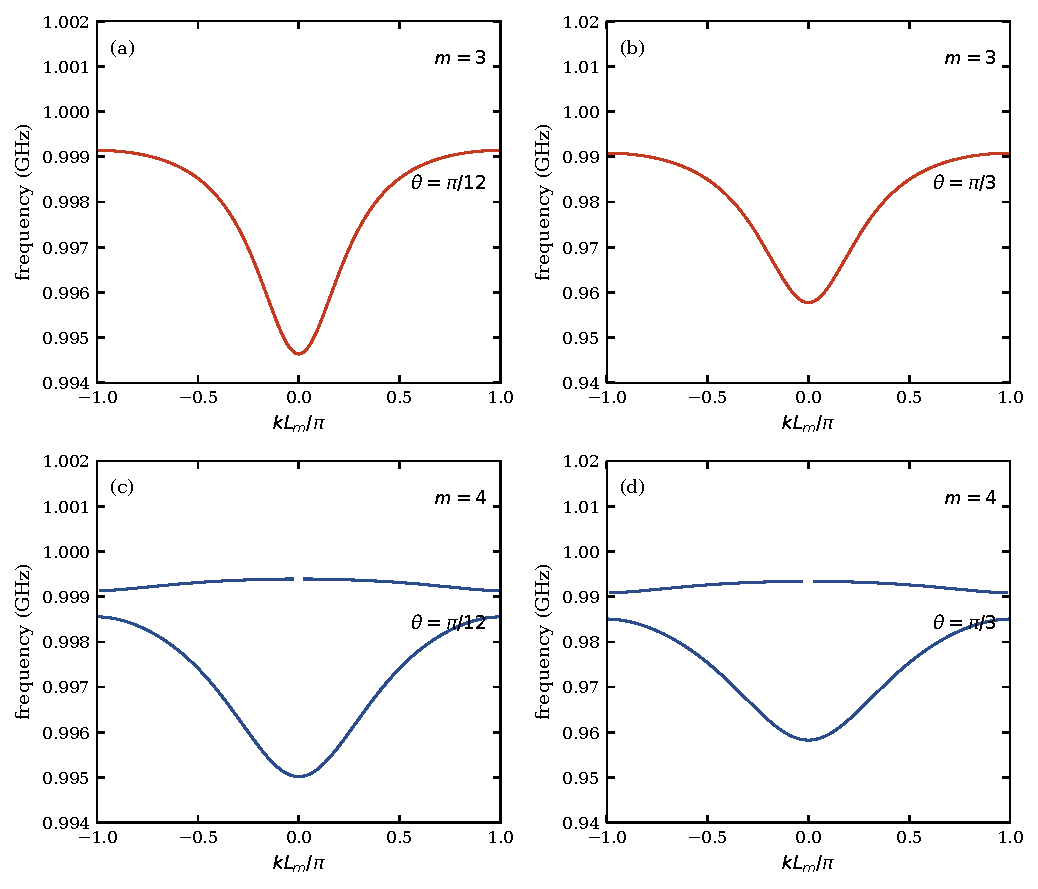
\includegraphics[width=0.95\linewidth]{figure_04/output/figure_04.pdf}
\caption{Reproducción de la Fig.~4. Zoom de los modos plasmon-polaritón.}
\end{figure}

\subsection{Figura 5}
$m=2$ y $m=3$ tienen un solo intervalo ($F_0=F_1=1$). A partir de $m=4$ hay splitting
sucesivo tipo Cantor. $\theta=\pi/3$ ensancha el espectro respecto a $\pi/12$.
El eje vertical del original está rotulado ``bandwidth (GHz)''; los valores
($0.994$--$1.000\,\mathrm{GHz}$ y $0.95$--$1.00\,\mathrm{GHz}$) son las frecuencias
de las subbandas permitidas, no $\Delta\nu$. Concordancia: \textbf{excelente}.

\begin{figure}[ht]
\centering
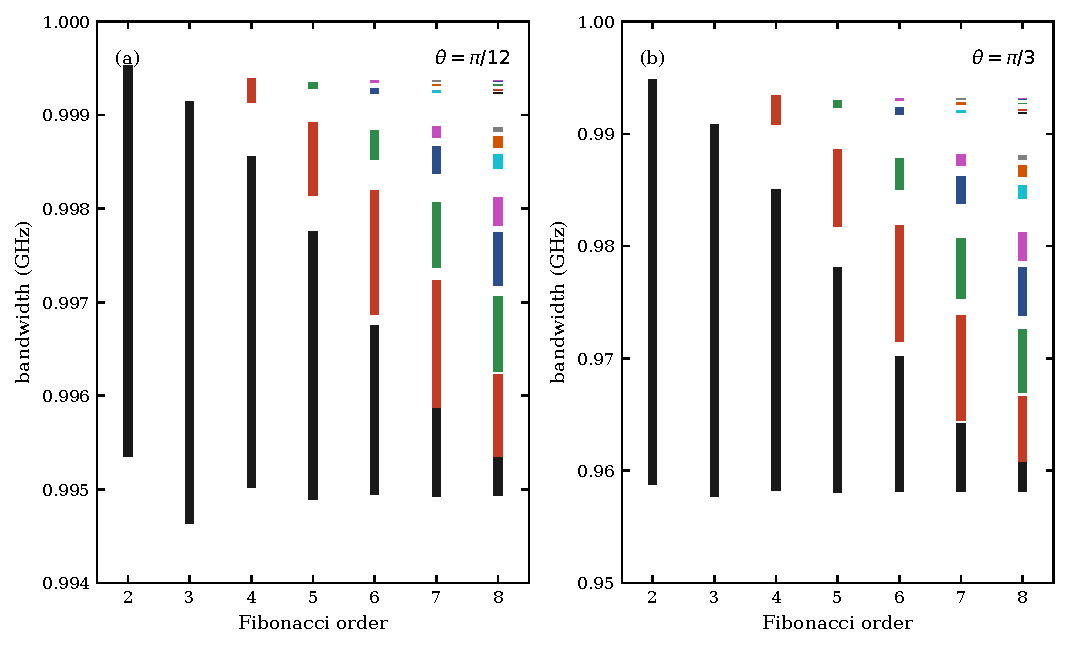
\includegraphics[width=0.95\linewidth]{figure_05/output/figure_05.pdf}
\caption{Reproducción de la Fig.~5. Intervalos permitidos frente al orden $m$.}
\end{figure}

\subsection{Figura 6}
El caption original está truncado. Se infieren los parámetros de las Figs.~3--5 y
$m=2,\ldots,7$. El original no grafica $\Delta\nu(\theta)$ como líneas que parten de
cero: grafica la \emph{frecuencia} de cada subbanda permitida frente a $\theta$,
con la región entre $\nu_{\min}(\theta)$ y $\nu_{\max}(\theta)$ rellena. A $\theta=0$
las ramas colapsan hacia $\nu_m=1\,\mathrm{GHz}$; al aumentar $\theta$ se abren hacia
abajo y se fragmentan según $F_{m-2}$. Concordancia: \textbf{buena}
(misma topología y paleta; parámetros no reiterados en el caption).

\begin{figure}[ht]
\centering
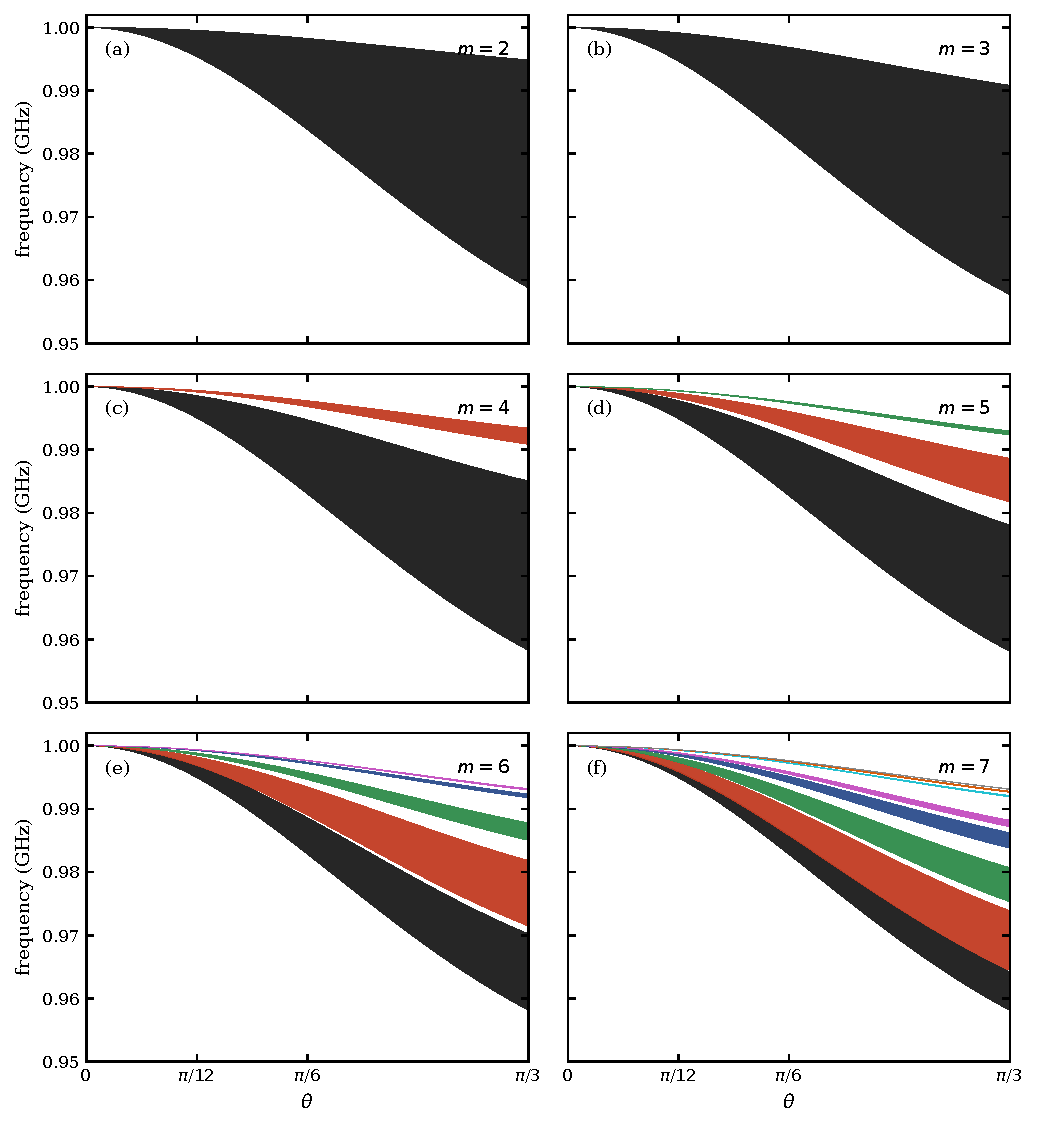
\includegraphics[width=0.85\linewidth]{figure_06/output/figure_06.pdf}
\caption{Reproducción de la Fig.~6 (parámetros inferidos). Frecuencia de las
subbandas plasmon-polaritón frente a $\theta$; el espesor de cada región es el
ancho de banda.}
\end{figure}

\section{Comparación con el paper original}

{\small
\begin{center}
\begin{tabular}{llp{4.2cm}p{4.6cm}}
\toprule
Fig.\ & Concordancia & Diferencia principal & Causa \\
\midrule
1 & Buena & Sin gaps a $\theta=0$ (físico) & Impedancia adaptada si $\omega_e=\omega_m$ \\
2 & Excelente & --- & $N=F_{m-2}$ exacto \\
3 & Buena & Comparación visual & No hay datos digitales del original \\
4 & Excelente & $\Delta\nu$ $\sim 20\%$ vs lectura visual & Lectura del impreso, no del dato \\
5 & Excelente & Eje rotulado bandwidth & En el PRB los valores son frecuencias \\
6 & Buena (inferida) & Caption incompleto & $m$ y plasma no reiterados; $\nu(\theta)$ relleno \\
\bottomrule
\end{tabular}
\end{center}
}

No se afirma coincidencia pixel a pixel: no hay vectorial del original.

\section{Análisis físico}

El splitting con $m$ es el de $F_{m-2}$ osciladores (capas B) acoplados por las capas A.
Si $a\gg b$ habría degeneración; aquí $a\sim b$ y se rompe.
Si $\nu_m$ es frecuencia permitida a $\theta=0$ (Figs.~1--2), el acoplamiento luz--plasmón
es fuerte y las bandas son dispersivas.
Si $\nu_m$ cae en el gap $\langle n\rangle=0$ (Figs.~3--6), el acoplamiento se debilita y
las bandas son esencialmente plasmónicas, casi planas, con espectro tipo Cantor.

\section{Análisis de convergencia}

Para el modo $m=3$, $\theta=\pi/3$, ventana $0.94$--$0.999\,\mathrm{GHz}$,
el ancho pasa de $0.03299\,\mathrm{GHz}$ (500 puntos) a $0.03310\,\mathrm{GHz}$
(16000 puntos). A partir de 2000 puntos la variación es menor que $0.2\%$.
El recuento de modos es estable. $c$ SI frente a $3\times 10^8\,\mathrm{m/s}$
cambia las frecuencias en $\sim 0.07\%$, por debajo de la resolución visual del original.

\section{Limitaciones y discrepancias}

\begin{itemize}
\item $q$ sin $\omega/c$ en el original: se restauró.
\item $c$ no dado.
\item Matriz de capa no escrita: se dedujo y se contrastó con (7)--(9).
\item Fig.~6: parámetros inferidos; el caption original está truncado.
\item Sin pérdidas, sin perfiles de campo, sin figuras TM.
\item No se ajustaron parámetros para ``parecerse'' al dibujo.
\end{itemize}

\section{Conclusiones}

El TMM con las ecuaciones del PRB~2010 reproduce las Figs.~1--5, incluido el recuento
$N_{\mathrm{modos}}=F_{m-2}$ y la dependencia angular del ancho de las subbandas planas.
La Fig.~6 reproduce la topología del original (regiones de $\nu$ vs $\theta$) con
parámetros inferidos del resto del artículo.
El proyecto es reproducible: configuración YAML, código, tests y figuras generadas
por scripts.

\appendix
\section{Unidades}
$\omega=2\pi\nu$, $\nu$ en GHz, longitudes en mm convertidas a SI.
No se mezcla $f$ con $\omega$.

\section{Cómo reproducir}
\texttt{pytest}; \texttt{python scripts/tmm/run\_all.py}; \texttt{make paper}.

\begin{thebibliography}{9}
\bibitem{Reyes2010}
E.~Reyes-Gómez, N.~Raigoza, S.~B.~Cavalcanti, C.~A.~A.~de Carvalho y L.~E.~Oliveira,
Phys.\ Rev.\ B \textbf{81}, 153101 (2010).
\bibitem{Reyes2009EPL}
E.~Reyes-Gómez, D.~Mogilevtsev, S.~B.~Cavalcanti, C.~A.~A.~de Carvalho y L.~E.~Oliveira,
EPL \textbf{88}, 24002 (2009).
\bibitem{Kohmoto1983}
M.~Kohmoto, L.~P.~Kadanoff y C.~Tang, Phys.\ Rev.\ Lett.\ \textbf{50}, 1870 (1983).
\bibitem{Veselago1968}
V.~G.~Veselago, Sov.\ Phys.\ Usp.\ \textbf{10}, 509 (1968).
\bibitem{Pendry1996}
J.~B.~Pendry, A.~J.~Holden, W.~J.~Stewart y I.~Youngs, Phys.\ Rev.\ Lett.\ \textbf{76}, 4773 (1996).
\bibitem{Pacheco2002}
J.~Pacheco, Jr., T.~M.~Grzegorczyk, B.-I.~Wu, Y.~Zhang y J.~A.~Kong,
Phys.\ Rev.\ Lett.\ \textbf{89}, 257401 (2002).
\bibitem{Li2003}
J.~Li, L.~Zhou, C.~T.~Chan y P.~Sheng, Phys.\ Rev.\ Lett.\ \textbf{90}, 083901 (2003).
\bibitem{Bruno2008}
A.~Bruno-Alfonso, E.~Reyes-Gómez, S.~B.~Cavalcanti y L.~E.~Oliveira,
Phys.\ Rev.\ A \textbf{78}, 035801 (2008).
\end{thebibliography}

\end{document}
